\section{Active Directory}
\begin{itemize}
  \item Active Directory (AD) ist ein Verzeichnisdienst (Datenbank), der von Microsoft entwickelt wurde.
  \item Verwendung für die zentrale Verwaltung von Computern, Servern, Benutzern, etc.
  \item führt die Authentifizierung und Autorisierung von Benutzern und Computern durch
  \begin{itemize}
    \item Überprüft die Anmeldedaten der Benutzer und legt ihre Zugriffsrechte fest
    \item Es basiert auf LDAP, NTLM, Kerberos (Microsofts Version), DNS und anderen Protokollen.
  \end{itemize}
  \item Strukturierung in Objekten
  \begin{itemize}
    \item Ressourcen (z. B. Drucker) \& Sicherheitsprinzipien (z. B. Benutzer, Gruppen, Computerkonten)
  \end{itemize}
  \item Organisationseinheiten
  \begin{itemize}
    \item Objekte innerhalb einer Domäne können in OUs gruppiert werden.
    \item OUs können einer Domäne eine Hierarchie verleihen. Dies vereinfacht die Verwaltung.
  \end{itemize}
  \item Logische Unterteilungen: forest, tree \& domain
\end{itemize}

\paragraph{Vorteile:}
\begin{itemize}
  \item Single-Sign On (Kerberos)
  \item Derselbe Benutzer kann sich mit seinem Domänenkennwort an jedem Computer anmelden, der mit der Domäne verbunden ist.
\end{itemize}

\subsection{Terminology}
\paragraph{Container}
\begin{itemize}
  \item Übergeordnetes Objekt für bestimmte Arten von AD-Objekten
  \item Forests, Domains, OUs, Sites, subnets
\end{itemize}
\paragraph{Domain}
\begin{itemize}
  \item Objekte werden immer in einer Domäne gesammelt
  \item Logische Gruppe von Netzwerkobjekten (Computer, Benutzer, Geräte)
  \item Identifiziert durch einen DNS-Namen (namespace)
\end{itemize}
\paragraph{Tree}
\begin{itemize}
  \item Sammlung von einer oder mehreren Domänen oder Trees
  \item Verbunden in einer transitiven Vertrauenshierarchie
\end{itemize}
\paragraph{Forest}
\begin{itemize}
  \item Einzelne Active Directory-Instanz
  \item Sammlung von Trees, die einen gemeinsamen globalen Katalog nutzen
  \item Sicherheitsabgrenzung (Security Boundary)
\end{itemize}

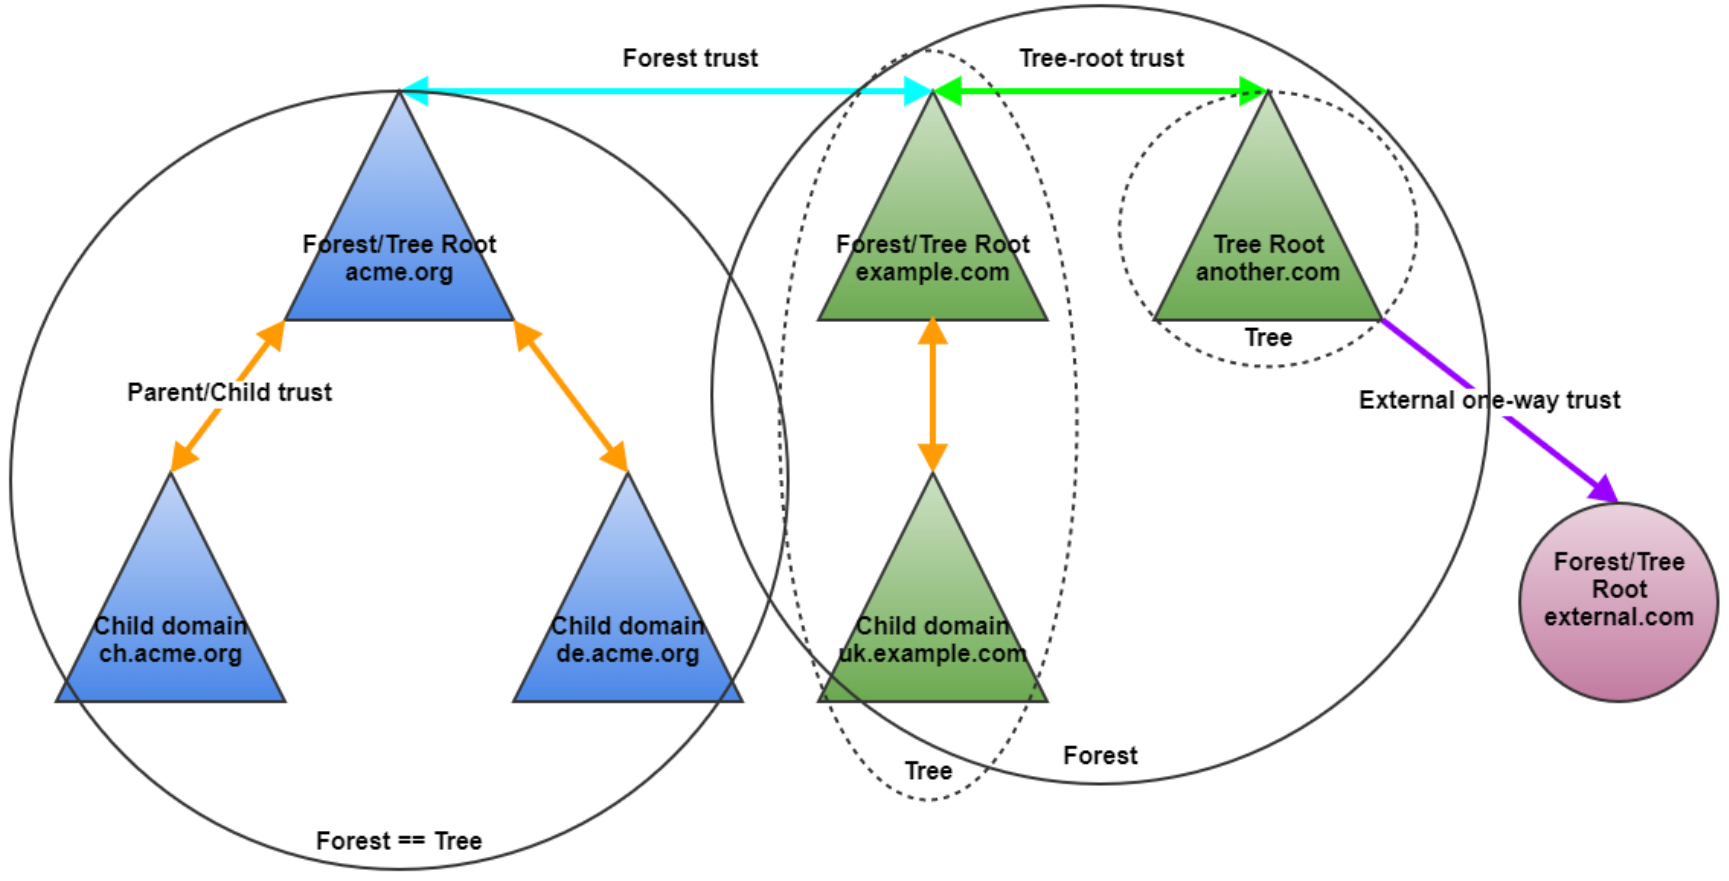
\includegraphics[width=0.75\linewidth]{ad-structure.png}

\subsection{Security Principals}
Ein security principal ist eine Einheit, die authentifiziert werden kann.
zum Beispiel ein User, eine Computer oder eine Gruppe.\\

Die SID (Security Identifier) identifiziert einen security principal eindeutig und die Zugangskontrolle basiert auf SIDs.\\

\includegraphics[width=\linewidth]{sid.png}

\subsection{Access Control List (ACL)}
Eine access control list (ACL) ist eine Liste von access control entries (ACE).
Ein ACE gibt die Zugriffsrechte an, die für diesen Trustee erlaubt, verweigert oder geprüft werden.
Der security descriptor für ein securable Object kann zwei Arten von ACLs enthalten:
\begin{itemize}
  \item \textbf{Discretionary Access Control (DACL)}: Eine Liste identifiziert die Trustees, denen der Zugriff auf ein sicheres Objekt erlaubt oder verweigert wird.
  \item \textbf{System Access Control (SACL)}: Ermöglicht Administratoren das Loggen von Zugriffsversuchen auf ein gesichertes Objekt.
\end{itemize}
\subsubsection{Beispiel}
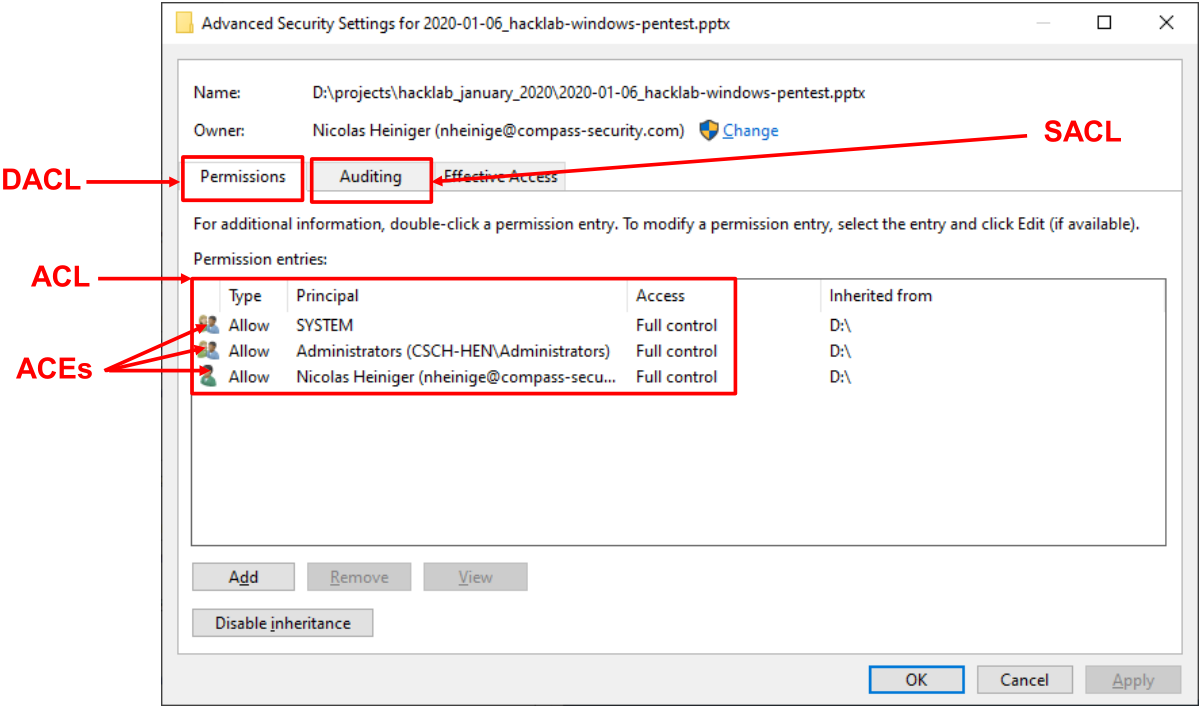
\includegraphics[width=\linewidth]{acl-example.png}

\subsection{Administratoren}
\paragraph{BUILTIN/Administrators}
Lokaler Admin Zugriff auf Domain Controller.
\paragraph{Domain Admins}
Administrativer Zugriff zu allen Ressourcen in der Domäne.
\paragraph{Enterprise Admins}
Existiert nur im Forest Root. Wird implizit zu "Domain Admins" jeder untergeordneten Domain hinzugefügt.
\paragraph{Schema Admins}
Kann das Domänen-/Forest Schema ändern
\paragraph{Server Operators}
Kann Domänenserver verwalten.
\paragraph{Account Operators}
Kann jeden Benutzer verwalten, der nicht zu einer "privilegierten" Gruppe gehört.

\subsection{Active Directory Threats}
Das Active Directory speichert den Passwort-Hash eines jeden Benutzers und den Computer-Hash eines jeden Computers. 
Die AD-Infrastruktur kann sehr komplex und daher schwer zu konfigurieren und sicher zu warten sein.
Ein gutes Ziel für Angreifer, denn wenn die AD kompromittiert ist, ist alles kompromittiert.\\

Häufige Fehlkonfigurationen und Fallstricke, die von Angreifern missbraucht werden können:
\begin{itemize}
  \item Keine Trennung des privilegierten Zugangs, z. B. hoch privilegierte Administratoren melden sich interaktiv bei Clients/Servern an.
  \item Dienst- (oder Benutzer-) Konten mit schwachen Passwörtern und SPN (Service Principal Names) gesetzt. Noch schlimmer, wenn die Wwnership verloren geht.
  \item Schwache Passwörter im Allgemeinen.
  \item Gleiches lokales Administrator-Passwort auf allen Computern.
  \item Wiederverwendung von Passwörtern im Allgemeinen.
  \item Anmeldeinformationen auf Shares (z.B. Skripte auf SYSVOL), auf die jeder Lese-/Schreibzugriff hat.
  \item Fehlen des least-privilege principle.
\end{itemize}

\subsection{Tools}
\paragraph{Active Directory Users \& Computers (ADUC)}
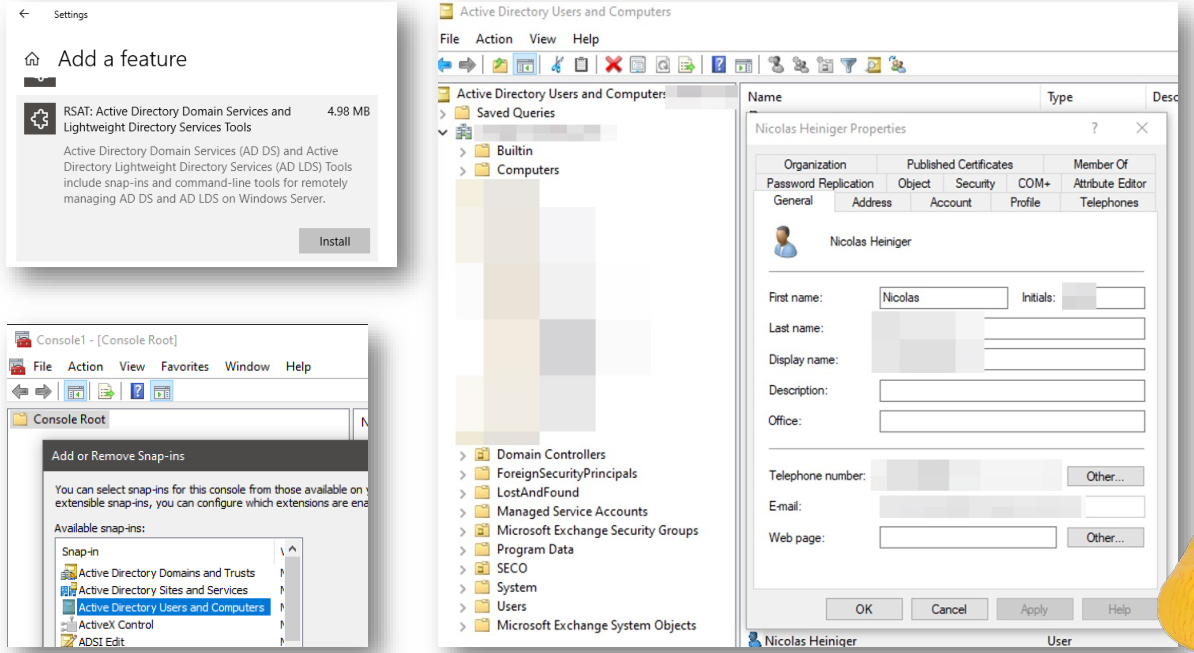
\includegraphics[width=\linewidth]{ADUC.png}

\paragraph{AD Explorer}
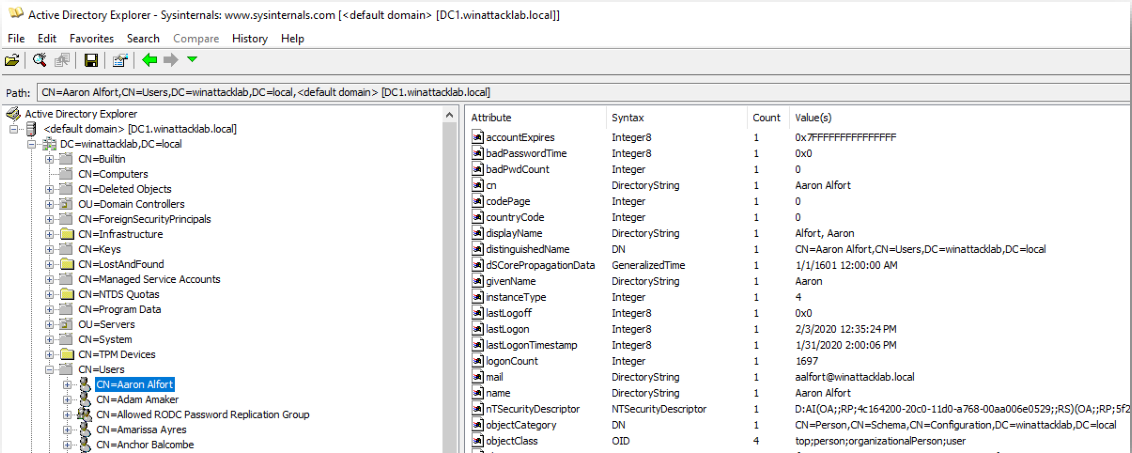
\includegraphics[width=\linewidth]{ad-explorr.png}\\
Sysinternals tool, wenn ADUC nicht vorhanden ist.\\
\textbf{Pro Tipp:}\\
\begin{itemize}
  \item Wenn Sie beim Herstellen der Verbindung nichts eingeben, verbinden Sie sich mit der aktuellen Domäne mit dem aktuellen Benutzer, ohne dass Sie ein Passwort eingeben müssen.
  \item Sie können Snapshots von einer Domäne machen und diese später offline analysieren
\end{itemize}

\paragraph{Net Tools}
\begin{lstlisting}
# info on local/domain user
net user alice [/domain]
# info on local/domain group
net localgroup Administrators
net group "Domain Admins" /domain
# list local/remote computer shares
net share
net view \\fileserver01
# list the password policy
net accounts
\end{lstlisting}

\paragraph{WMI}
WMI kann:
\begin{itemize}
  \item Laufende Prozesse auflisten
  \item Installierte Antivirenprogramme auflisten
  \item Installierte Updates auflisten
  \item Benutzer, Computer und Gruppen in der Domäne auflisten
  \item Dateien und Registry lesen
  \item Prozess erstellen (lokal oder remote)
  \item RDP aktivieren (lokal oder remote)
\end{itemize}

Kann via CLI verwendet werden:
\begin{lstlisting}
  wmic NTDOMAIN GET DomainControllerAddress,DomainName,Roles /VALUE
  wmic process call create "cmd.exe /c calc.exe"
  wmic /node:REMOTEHOST path Win32_TerminalServiceSetting where AllowTSConnections="0" call SetAllowTSConnections "1"
\end{lstlisting}

\subsubsection{Ping Castle}
Ping Castle ist ein Tool zur schnellen Bewertung des Sicherheitsniveaus von Active Directory mit einer Methodik, die auf einer Risikobewertung und einem Reifegradrahmen basiert.\\
\paragraph{Haupt-Features}
\begin{itemize}
  \item Gesundheitscheck der Domäne
  \item Kartographie der Domänen-Trusts
  \item Scanner für verschiedene Einstellungen (LAPS, Lokale Admins, Shares, SMB, Spooler)
\end{itemize}

\subsection{Azure Active Directory}
\begin{itemize}
  \item Gleiche Idee wie bei Active Directory vor Ort
  \item Zentral verwaltete Domäne für Enterprise Admins
  \item GPO nicht zu 100\% in Azure verfügbar
  \item Richtlinie jetzt im Endpoint Manger Interface von Azure
  \item Bedingte Zugriffskontrolle (MDM, Mobile Device Management)
\end{itemize}



\subsection{Active Directory GPO}
\subsubsection{SYSVOL}
Das Systemvolume (SYSVOL) ist ein spezielles Verzeichnis auf jedem DC.
Es besteht aus mehreren Ordnern, von denen einer shared ist und als SYSVOL-Freigabe bezeichnet wird.\\

Der Standardspeicherort für den shared Ordner ist \%SYSTEMROOT/SYSVOL/sysvol, obwohl Sie dies während des DC-Promotionsprozesses oder jederzeit danach ändern können.
SYSVOL setzt sich aus Ordnern zusammen. 
Die Ordner werden zum Speichern verwendet:
\begin{itemize}
  \item Group Policy templates (GPTs), die über SYSVOL-Replication repliziert werden. Der Group Policy container (GPC) wird über die Active Directory-Replication repliziert.
  \item Skripte, wie z. B. Startskripte, die in einem GPO referenziert werden.
\end{itemize}

\subsubsection{Group Policy Object (GPO)}
Ein GPO ist eine virtuelle Sammlung von Ploicies. 
Ein GPO hat einen eindeutigen Namen, wie eine GUID.\\

Group Policy settings sind in einem GPO enthalten. 
Ein GPO kann policy settings im Dateisystem und im Active Directory darstellen. 
Die GPO-Einstellungen werden von den Clients anhand der hierarchischen Natur von Active Directory ausgewertet.\\

Zum Erstellen von Gruppenrichtlinien kann ein Administrator den Gruppenrichtlinienobjekt-Editor verwenden, der ein eigenständiges Tool sein kann. 
Es wird jedoch empfohlen, den Gruppenrichtlinien-Objekteditor als Erweiterung zu einem Active Directory-bezogenen MMC-Snap-In zu verwenden.

\subsubsection{Folder \& File Policy}
Create a Folder or a File on every computer in the domain.
Can be applied to all or a subset of all computer.

\subsubsection{Update GPO on Computers}
\paragraph{Local computer}
Run ``gpupdate /force'' in cmd.

\paragraph{Remote}
Run 
\begin{lstlisting}
  $computers = Get-ADComputer -Filter *
  $computers |ForEach-Object -Process {Invoke-GPUpdate -Computer $_.name -RandomDelayInMinutes 0 -Force}
\end{lstlisting}
